\documentclass{oci}
\usepackage[utf8]{inputenc}
\usepackage{lipsum}
\usepackage{tikz}
\usepackage[dvipsnames]{xcolor}

\definecolor{pedro}{HTML}{FE5F55}
\definecolor{amigo}{HTML}{5995ED}

\newcommand{\cine}{
    % Row 1: 0 1 1 1 0
    \fill[black] (1,3) rectangle (2,4);
    \fill[black] (2,3) rectangle (3,4);
    \fill[black] (3,3) rectangle (4,4);

    % Row 2: 1 0 0 1 1
    \fill[black] (0,2) rectangle (1,3);
    \fill[black] (3,2) rectangle (4,3);
    \fill[black] (4,2) rectangle (5,3);

    % Row 3: 1 1 1 0 1
    \fill[black] (0,1) rectangle (1,2);
    \fill[black] (1,1) rectangle (2,2);
    \fill[black] (2,1) rectangle (3,2);
    \fill[black] (4,1) rectangle (5,2);

    % Row 4: 0 0 1 0 1
    \fill[black] (2,0) rectangle (3,1);
    \fill[black] (4,0) rectangle (5,1);


    \foreach \x in {1, 2, 3, 4, 5} {
        \node[above] at (\x-1+0.5, 4) {\small\x};
    }
    \foreach \y in {1, 2, 3, 4} {
        \node[left] at (0, 4-\y+0.5) {\small\y};
    }
    \draw (0,0) grid (5,4);
}

\title{Cine}

\begin{document}
\begin{problemDescription}
    Pedro y sus $K$ amigos llegaron tarde al cine y
    para su desagradable sorpresa se dieron cuenta
    de que la mayoría de los asientos ya estaban ocupados.
    %
    Aunque puede que ya no sea posible encontrar
    asientos contiguos, a Pedro le gustaría sentarse
    lo más cerca posible de sus amigos para disfrutar
    juntos de la película.

    Los asientos en el cine están distribuidos en una
    grilla de $N$ filas y $M$ columnas.
    %
    Las filas son numeradas de arriba hacia abajo
    de $1$ a $N$ y las columnas de izquierda a derecha
    de $1$ a $M$.
    %
    La posición de un asiento se representa con un par
    $(x, y)$ donde $x$ representa la columna e $y$ la fila.
    %
    Pedro quiere encontrar una configuración de asientos
    de modo que la distancia entre él y su amigo más
    lejano sea la mínima posible.
    %
    La distancia entre Pedro y un amigo se define
    como el máximo entre la distancia horizontal y vertical.
    %
    Específicamente, si Pedro está sentado en la posición
    $(x_p, y_p)$ y su amigo $k$-ésimo en la posición
    $(x_k, y_k)$, la distancia entre ellos se define como
    $\max(|x_p - x_k|, |y_p - y_k|)$.
    %
    Llamaremos a la distancia entre pedro y su amigo más
    lejano la \emph{distancia grupal}.

    La siguiente imagen muestra un ejemplo para un cine
    con $4$ filas y $5$ columnas.
    %
    La cantidad de amigos es $K=3$ y se marca con negro
    los asientos que están ocupados.
    %
    La imagen muestra una configuración con Pedro sentado en
    la posición $(3, 2)$ (marcado con una cruz) y
    con sus amigos sentados en las posiciones $(2, 2)$, $(4, 3)$ y $(4, 4)$
    (marcados con un círculo).
    %
    En este escenario, la distancia entre Pedro y su amigo
    más lejano (el amigo en la posición $(4, 4)$) es $2$,
    es decir, la distancia grupal es $2$.
    %
    Esta distancia es además mínima, pues no hay ninguna
    otra configuración donde la distancia grupal
    sea menor que $2$.

    \begin{figure}[h]
        \centering
        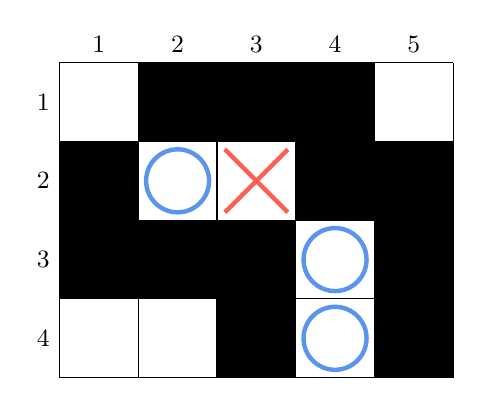
\begin{tikzpicture}
            % \fill[amigo] (1,2) rectangle (2,3);
            % \fill[pedro] (2,2) rectangle (3,3);
            % \fill[amigo] (3,1) rectangle (4,2);
            % \fill[amigo] (3,0) rectangle (4,1);

            \draw[ultra thick, amigo] (1.5,2.5) circle(0.4);
            \draw[ultra thick, pedro] (2.1, 2.1) -- (2.9, 2.9);
            \draw[ultra thick, pedro] (2.1, 2.9) -- (2.9, 2.1);
            \draw[ultra thick, amigo] (3.5,1.5) circle(0.4);
            \draw[ultra thick, amigo] (3.5,0.5) circle(0.4);


            \cine
        \end{tikzpicture}
        % \caption{Una posible asignación optima para el Cine anterior si Pedro tiene $K=3$ amigos.}
    \end{figure}

    Pedro está muy estresado pues la película está por comenzar y
    no sabe qué asientos comprar así que te ha pedido ayuda.
    %
    Dada la descripción del cine y cuáles asientos están ocupados,
    tu tarea es encontrar la mínima distancia grupal posible.
    %y su amigo más lejano, teniendo en cuenta que el puede elegir su propio asiento y la de sus $K$ amigos entre los asientos disponibles.

\end{problemDescription}

\begin{inputDescription}
La primera línea contiene tres enteros $N$, $M$ y $K$
($1 \leq N \cdot M \leq 10^6$, $1 \leq K \leq N \cdot M - 1$)
que representan respectivamente la cantidad de filas, la cantidad de columnas,
y la cantidad de amigos que tiene Pedro.

Cada una de las siguientes $N$ líneas contiene $M$ enteros.
%
El entero $x$-ésimo en la línea $y$-ésima describe el asiento
en la posición $(x, y)$.
%
El entero será $0$ si el asiento está disponible o $1$ si
está ocupado.

Se garantiza que la cantidad total de ceros es mayor o igual a $K+1$,
es decir, siempre es posible sentar a Pedro y a todos sus amigos.
\end{inputDescription}

\begin{outputDescription}
La salida debe contener un único entero correspondiente
a la distancia grupal mínima posible.
\end{outputDescription}

\begin{scoreDescription}
  \subtask{10} Se probarán varios casos de prueba donde $N\leq 20$ y $M \leq 20$.
  \subtask{20} Se probarán varios casos de prueba donde $N \cdot M \leq 5000$.
  \subtask{20} Se probarán varios casos de prueba donde $N = 1$.
  \subtask{50} Se probarán varios casos de prueba sin restricciones adicionales.
\end{scoreDescription}

\begin{sampleDescription}
\sampleIO{sample-1}
\end{sampleDescription}

\end{document}
